% Document class and parameters %
\documentclass[10pt,a4paper]{article}

% Document packages %
\usepackage{graphicx}
\usepackage{biblatex}
\usepackage{parskip}
\usepackage{listings}
\usepackage{caption}
\usepackage{subcaption}
\usepackage{amsmath}
\usepackage[most]{tcolorbox}
\usepackage{multicol}
\usepackage{nccmath}

%%%%%%%%%%%%%%%%%%%%%%%%%%%%%%%%%%%%%%%%%%%%%%%%%%%%%%%%%%%%%%%%%%%%%%%%%%%%%%%%%%%%%%%%%%%%%%%%%%%%%%%%%%
% Parameters %
\lstset{basicstyle=\ttfamily, breaklines = true, tabsize=2}
\graphicspath{{./Images/}}
\setlength{\parskip}{1em}

%%%%%%%%%%%%%%%%%%%%%%%%%%%%%%%%%%%%%%%%%%%%%%%%%%%%%%%%%%%%%%%%%%%%%%%%%%%%%%%%%%%%%%%%%%%%%%%%%%%%%%%%%%

% Document Body %
\begin{document}
\begin{titlepage}
	\centering
	{\scshape\LARGE ELEC40001 \par}
	\vspace{1cm}
	{\scshape\Large Mathematics: Year 1 \par}
	\vspace{1.5cm}
	{\huge\bfseries Orthogonal subspaces, Projection and Least Squares\par}
	\vspace{2cm}
	{\Large\ Xin Wang }
	\vfill
	{\large \today\par}
\end{titlepage}

%%%%%%%%%%%%%%%%%%%%%%%%%%%%%%%%%%%%%%%%%%%%%%%%%%%%%%%%%%%%%%%%%%%%%%%%%%%%%%%%%%%%%%%%%%%%%%%%%%%%%%%%%%

\begin{abstract}
Sometimes the matrix system $A \textbf{\underbar{x}} = \textbf{\underbar{b}}$ is inconsistent and
does not have a solution. For example, satellite trajectory projections shown in the form of matrix systems sometimes do
not have exact solutions. There are certain methods available to find an \textbf{approximate} solution when an exact
solution does not exist.
\end{abstract}

\tableofcontents
\pagebreak

%%%%%%%%%%%%%%%%%%%%%%%%%%%%%%%%%%%%%%%%%%%%%%%%%%%%%%%%%%%%%%%%%%%%%%%%%%%%%%%%%%%%%%%%%%%%%%%%%%%%%%%%%%
% Sections Body %
\section{Orthogonal Subspaces}

As previously mentioned, the dot product measures the amount of one vector goes in the direction of
each other. The dot product can be used to find if two vectors are orthogonal to each other. Two
vectors are \textbf{perpendicular} when dot product is zero:
\begin{align*}
	\textbf{v}*\textbf{w}=\textbf{v}^T*\textbf{w}=0 \\
	\left \| \textbf{v}\right \|^2*\left \| \textbf{w}\right\|^2=\left \| \textbf{v+w} \right \|^2
\end{align*}

\begin{tcolorbox}[breakable,colback=white]
Two subspaces V and W of a vector space are \textbf{orthogonal} if every vector \textbf{v} in set V is
perpendicular to every vector \textbf{w} in set W. $$v^T*w=0$$ for all \textbf{v} in V and all
\textbf{w} in W.
\end{tcolorbox}

\begin{figure} [h!]
	\centering
	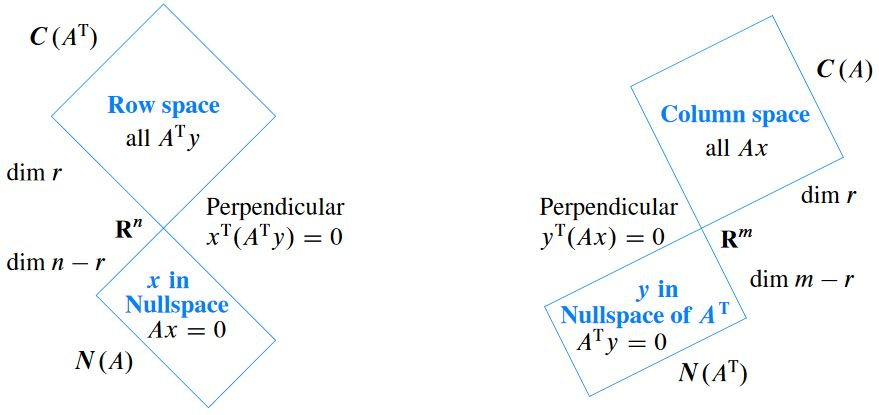
\includegraphics[scale=0.6]{Fundasub.JPG}
\end{figure}

The “big picture” of this chapter is that:
\begin{itemize}
    \item Row space $C(A^T)$ is perpendicular to null space of $N(A)$
    \item Column space $C(A)$ is perpendicular to null space of $N(A^T)$
\end{itemize}

Consider a wall and a floor as planes in $\Re^3$. Both are orthogonal to each other but they are not
orthogonal subspaces.
\begin{itemize}
    \item There are diagonal vectors in the wall that are not orthogonal to any vectors in the floor.
    \item The line of intersection is in both the floor and the wall. A vector can never be
    orthogonal to itself unless it is the zero vector.
\end{itemize}
\begin{tcolorbox}[breakable,colback=white]
	For two subspaces to be orthogonal, there must be \textbf{only} the zero vector at the intersection:
	$$ 
		V \cap W = \{\textbf{\underbar{0}}\} 
	$$
\end{tcolorbox}

%%%%%%%%%%%%%%%%%%%%%%%%%%%%%%%%%%%%%%%%%%%%%%%%%%%%%%%%%%%%%%%%%%%%%%%%%%%%%%%%%%%%%%%%%%%%%%%%%%%%%%%%%%
\subsection{Null space perpendicular to row space}

The null space of matrix $A$ is the set of all vectors $x$ for which $Ax = 0$. The product of the
matrix $A$ and the vector $x$ can be written in terms of the dot product of vectors: 
\begin{align*}
	A \textbf{x} = 
	\begin{bmatrix}
		\textbf{r}_1.x \\
		\textbf{r}_2.x \\
		. \\
		. \\
		. \\
		\textbf{r}_m.x
	\end{bmatrix}
\end{align*}
where $r_1,\dots,r_m$ are the row vectors of $A$. 

In order of the definition of null space to be satisfied, \textbf{$x$ has to be perpendicular to
each of the row vectors of $A$ ($\text{dot product} = 0$) in order for $Ax = 0$}. It follows that the null space of A is the orthogonal complement to the row space.


\begin{tcolorbox}[breakable,colback=white]
Every vector $\textbf{x}$ in null space is perpendicular to every row of $\textbf{A}$ due to the
fundamental definition of the null space where $Ax=0$. The null space $N(A)$ and row space $C(A^T)$ are orthogonal subspaces of $\Re^n$.
\end{tcolorbox}

\textbf{Example 1}: Show the null space and row space are orthogonal subspaces of $\Re^3$ in matrix $A$:
$$A= \begin{bmatrix}
	1 & 2 & 5\\ 
	2 & 4 & 10
	\end{bmatrix} $$

\begin{enumerate}
	\item Find the rank of the matrix:
	
	Matrix has rank of 1 since rows below first row are all multiples of the first row.
	\begin{align*}
		\text{Row space} = \textbf{C}(A^T)=k*
		\begin{bmatrix}
			1 \\
			2 \\
			5
		\end{bmatrix}
	\end{align*}
	\item Find the dimension of the row space: 
	\begin{align*}
		\text{dim }\textbf{C}(A^T) = 1 = \text{rank}(A)
	\end{align*}
	\item Find the dimension of the null space:  
	\begin{align*}
		\text{dim }\textbf{N}(A) = n-r = \text{rank}(A)
	\end{align*}
	\item Find the null space:
	\begin{itemize}
		\item Find the reduced row echelon form:
		\begin{ceqn}
		\begin{equation*}
			A \sim 
			\begin{bmatrix}
				1 & 2 & 5 \\
				0 & 0 & 0
			\end{bmatrix} \\
			\Rightarrow A\textbf{\underbar{x}}=\textbf{\underbar{0}} \rightarrow x_1 + 2x_2 + 5x_3 = 0
		\end{equation*}
		\end{ceqn}
		\item Find the special solutions:
		\begin{equation*} 
			\begin{bmatrix}
				-2 \\
				1 \\
				0
				\end{bmatrix} \textrm{ and } \begin{bmatrix}
					-5 \\
					0 \\
					1
					\end{bmatrix}
		\end{equation*}
		\item Find the linear linear combinations that form the null space:
		\begin{equation*} 
			\begin{bmatrix}
				-2 \\
				1 \\
				0
				\end{bmatrix}^T*\begin{bmatrix}
					1 \\
					2 \\
					5
					\end{bmatrix}=0\textrm{ and } \begin{bmatrix}
					-5 \\
					0 \\
					1
					\end{bmatrix}^T*\begin{bmatrix}
						1 \\
						2 \\
						5
						\end{bmatrix} = 0
		\end{equation*} 
	\end{itemize}
	\item Results show every vector in row space is orthogonal to every vector in the null space.
\end{enumerate}

%%%%%%%%%%%%%%%%%%%%%%%%%%%%%%%%%%%%%%%%%%%%%%%%%%%%%%%%%%%%%%%%%%%%%%%%%%%%%%%%%%%%%%%%%%%%%%%%%%%%%%%%%%
\subsection{Left null space orthogonal to column space}

\begin{tcolorbox}[breakable,colback=white]
	Every vector $\textbf{y}$ in the null space of $A^T$ i.e. left null space is perpendicular to
	every column of $A$. The left null space $N(A^T)$ and the column space $C(A)$ are orthogonal in
	$\Re^m$.
\end{tcolorbox}

%%%%%%%%%%%%%%%%%%%%%%%%%%%%%%%%%%%%%%%%%%%%%%%%%%%%%%%%%%%%%%%%%%%%%%%%%%%%%%%%%%%%%%%%%%%%%%%%%%%%%%%%%%
\section{Projection}

When $b$ is projected onto a line, its \textbf{projection} $p$ is the part of $b$ along that line.
If $\textbf{b}$ is projected onto a plane, $p$ is the part in that plane denoted $P\: \textbf{b}$
\begin{figure} [h!]
	\centering
	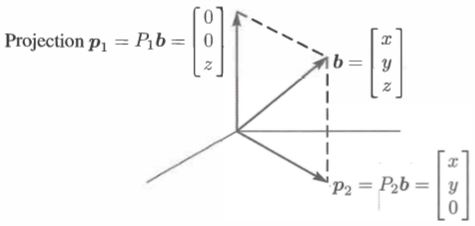
\includegraphics[scale=0.8]{Projection.JPG}
	\caption{Projection visualised}
\end{figure}

%%%%%%%%%%%%%%%%%%%%%%%%%%%%%%%%%%%%%%%%%%%%%%%%%%%%%%%%%%%%%%%%%%%%%%%%%%%%%%%%%%%%%%%%%%%%%%%%%%%%%%%%%%
\subsection{Properties of $A^T\:A$}

A matrix that was covered previously. This matrix is a square matrix of dimensions $n \times n$ and
symmetric. Its null space is of particular interest especially if the square matrix is not invertible.

Given:
$$
	A\textbf{\underbar{x}}=\textbf{\underbar{b}}
$$
multiply by $A^T$ to form a new equation: 
\begin{align*}
	A^T \times A\hat{\textbf{\underbar{x}}} &= A^T \times \textbf{\underbar{b}} \\
	\Rightarrow A^T\: A \hat{\textbf{\underbar{x}}} &= A^T\: \textbf{\underbar{b}}
\end{align*}

Note $\textbf{\underbar{x}}$ is changed into $\hat{\textbf{\underbar{x}}}$ because the result is \textbf{an
approximation} as the exact solution \textbf{\underbar{x}} cannot be found. 

\begin{tcolorbox}[breakable,colback=white]
	The result of $A^T\:A$ is a square matrix and symmetric but \textbf{not always invertible}. The
	invertibility of $A^T\:A$ depends on $A$ having independent columns i.e.
	$N(A)=\textbf{\underbar{0}}$
	\begin{equation*} 
	N(A^T\:A)=N(A) \textrm{ and } rank(A^T\:A)=rank(A) 
	\end{equation*}
\end{tcolorbox}


%%%%%%%%%%%%%%%%%%%%%%%%%%%%%%%%%%%%%%%%%%%%%%%%%%%%%%%%%%%%%%%%%%%%%%%%%%%%%%%%%%%%%%%%%%%%%%%%%%%%%%%%%%
\subsection{Projection in 1D}

The interest in projection is due to the point given by $\textbf{\underbar{p}}$, the projection of
$\textbf{\underbar{b}}$ onto $\textbf{\underbar{a}}$, this is the point on $\textbf{\underbar{a}}$
nearest to $\textbf{\underbar{b}}$. As mentioned previously if the exact solution
$\textbf{\underbar{b}}$ is not available, an approximation can be made by taking the nearest point
on $\textbf{\underbar{a}}$ as an approximation  and $\textbf{\underbar{e}} \neq
\textbf{\underbar{0}}$ is the resulting error. \par
\begin{figure} [h!]
	\centering
	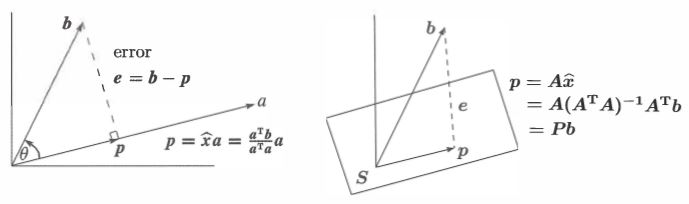
\includegraphics[scale=0.7]{Projection_1D.JPG}
	\caption{Projection onto a line}
\end{figure}
The key to projection is te orthogonality property - the point $\textbf{\underbar{p}}$ on line
$\textbf{\underbar{a}}$ that is closest to $\textbf{\underbar{b}}$. As $\textbf{\underbar{a}}$ is
only an approximation of $\textbf{\underbar{b}}$, there is an resulting error
$\textbf{\underbar{e}}$:
$\textbf{\underbar{e}}=\textbf{\underbar{b}}-\hat{\textbf{x}}\textbf{\underbar{a}}$ \par 
Projection is usually defined as: $\textbf{\underbar{p}} = \lambda\textbf{\underbar{a}}$ with
$\lambda$ can be defined as: 
\begin{align*}
	\lambda =
	\frac{\textbf{\underbar{a}}*\textbf{\underbar{b}}}{\textbf{\underbar{a}}*\textbf{\underbar{a}}}=\frac{\textbf{\underbar{a}}^T*\textbf{\underbar{b}}}{\textbf{\underbar{a}}^T*\textbf{\underbar{a}}}
\end{align*}
hence simplify:
\begin{align*}
	\textbf{\underbar{p}}=\frac{\textbf{\underbar{a}}^T*\textbf{\underbar{b}}}{\textbf{\underbar{a}}^T*\textbf{\underbar{a}}}*\textbf{\underbar{a}}=\frac{(\textbf{\underbar{a}}^T*\textbf{\underbar{b}})*\textbf{\underbar{a}}}{\textbf{\underbar{a}}^T*\textbf{\underbar{a}}}
	=
	\frac{\textbf{\underbar{a}}*\textbf{\underbar{a}}^T}{\textbf{\underbar{a}}^T*\textbf{\underbar{a}}}*\textbf{\underbar{b}}=P*\textbf{\underbar{b}}
\end{align*}
where $P$ is the \textbf{Projection Matrix} defined as:
$$P=\frac{\textbf{\underbar{a}}*\textbf{\underbar{a}}^T}{\textbf{\underbar{a}}^T*\textbf{\underbar{a}}}$$

%%%%%%%%%%%%%%%%%%%%%%%%%%%%%%%%%%%%%%%%%%%%%%%%%%%%%%%%%%%%%%%%%%%%%%%%%%%%%%%%%%%%%%%%%%%%%%%%%%%%%%%%%%
\subsection{Projection in a subspace (2D or higher)}

As stated earlier, if $A \textbf{\underbar{x}}=\textbf{\underbar{b}}$ has no solutions, the closest
solution can be found by considering $A \textbf{\underbar{x}}$ in the column space $C(A)$ and
find $\textbf{\underbar{p}}$ which is the closest vector in $C(A)$ to $\textbf{\underbar{b}}$: 
$$
	A \hat{\textbf{\underbar{x}}} = \textbf{\underbar{p}}
$$
where:
\begin{itemize}
	\item $\textbf{\underbar{p}}$ is the nearest point to $\textbf{\underbar{b}}$ in the plane
	\item The error is defined as $\textbf{\underbar{e}}=\textbf{\underbar{b}}-\textbf{\underbar{p}} = \textbf{\underbar{b}}-A \hat{\textbf{\underbar{x}}}$
\end{itemize} 

\begin{tcolorbox}[breakable,colback=white]
If $\textbf{\underbar{p}}$ is in the column space, the error $\textbf{\underbar{e}}$ must be in
$N(A^T)$, orthogonal to the column space.
\end{tcolorbox}
\begin{tcolorbox}[breakable,colback=white]
	The process involving projection is summarised in three steps:
	\begin{enumerate}
		\item Find the vector $\hat{\textbf{x}}$:
		$$A^T*A*\hat{\textbf{x}}=A^T*\textbf{\underbar{b}}$$
		$$\hat{\textbf{x}}=(A^T*A)^{-1}*A^T*\textbf{b}$$
		\begin{itemize}
			\item The matrix $A^T*A$ is symmetric 
			\item Invertible if columns are independent 
		\end{itemize}
		\item Projection $\textbf{p}$ of $\textbf{b}$ onto subspace:
		$$\textbf{p}=A*\hat{\textbf{x}}=A(A^T*A)^{-1}*A^T*\textbf{b}$$
		\item Projection Matrix $\textbf{P}$:
		$$\textbf{P}=A(A^T*A)^{-1}*A^T$$
	\end{enumerate}
\end{tcolorbox}

%%%%%%%%%%%%%%%%%%%%%%%%%%%%%%%%%%%%%%%%%%%%%%%%%%%%%%%%%%%%%%%%%%%%%%%%%%%%%%%%%%%%%%%%%%%%%%%%%%%%%%%%%%
\subsection{Least-squares method - Linear Regression}

When $Ax=b$ has no solution, this is usually due to there being too many equations e.g. $A$ has more
rows than columns i.e. more equations than unknowns.

\begin{tcolorbox}[breakable,colback=white]
When $Ax=b$ has no solution, multiply by $A^T$ and solve the equation:
$$
	A^T*A*\hat{x}=A^T*b
$$
where $\hat{x}$ is the \textbf{least-square solution} i.e. where the error $e$ is the smallest.
\end{tcolorbox}

\textbf{Example 1:} Find the quadratic line of best fit with the following points:
\begin{multicols}{2}
	\begin{itemize}
		\item $(x,y) = (-1,1)$
		\item $(x,y) = 	(0,3)$
		\item $(x,y) = (1,4)$
		\item $(x,y) = (2,0)$
	\end{itemize}
\end{multicols}
where $y(x)$ is the trajectory of the object thrown at an angle - a parabolic curve: $y=ax^2+bx+c$ - subjected to gravity.
\begin{enumerate}
	\item Formulate the problem - identify the parameters:
	\begin{itemize}
		\item at $(-1,1)$: $1=a-b+c$
		\item at $(0,3)$: $3=0a+0b+c$
		\item at $(1,4)$: $4=a+b+c$
		\item at $(2,0)$: $0=4a+2b+c$
	\end{itemize}
	\item Form matrix notation:
	\begin{align*}
		A \textbf{\underbar{x}} &= \textbf{\underbar{b}} \\
		\Rightarrow \begin{bmatrix}
			1&-1&1\\
			0&0&1\\
			1&1&1\\
			4&2&1
		\end{bmatrix}\textbf{\underbar{x}} &= \begin{bmatrix}
			1\\
			3\\
			4\\
			0
		\end{bmatrix}
	\end{align*}
	\item Verify that it has no solutions: Not full rank.
	\item Form equation: $A^T\:A\hat{\textbf{\underbar{x}}}=A^T*\textbf{\underbar{b}}$:
	$$A^T*A*\hat{\textbf{\underbar{x}}}=
	\begin{bmatrix}
		1&0&1&4\\
		-1&0&1&2\\
		1&1&1&1\\
	\end{bmatrix}*
	\begin{bmatrix}
		1&-1&1\\
		0&0&1\\
		1&1&1\\
		4&2&1
	\end{bmatrix}*\hat{\textbf{\underbar{x}}} = 
	\begin{bmatrix}
		1&0&1&4\\
		-1&0&1&2\\
		1&1&1&1\\
	\end{bmatrix}*\begin{bmatrix}
		1\\
		3\\
		4\\
		0
	\end{bmatrix}=A^T*\textbf{\underbar{b}}$$
	\item Simplify:
	$$\begin{bmatrix}
		18&8&6\\
		8&6&2\\
		6&2&4
	\end{bmatrix}*\hat{\textbf{\underbar{x}}} = \begin{bmatrix}
		5\\
		3\\
		8
	\end{bmatrix}$$
	\item Verify the columns are independent: Not multiples of each other.
	\item Invert to obtain $\hat{\textbf{\underbar{x}}}$:
	$$\hat{\textbf{\underbar{x}}}=(A^T*A)^{-1}*(A^T*\textbf{\underbar{b}})=\frac{1}{20}
	\begin{bmatrix}
		5&-5&-5\\
		-5&9&3\\
		-5&3&11
	\end{bmatrix}*
	\begin{bmatrix}
		5\\
		3\\
		8
	\end{bmatrix}=
	\begin{bmatrix}
		-1.5\\
		1.3\\
		3.6
	\end{bmatrix}$$
	\item Form the resulting equation:
	$$y=-1.5x^2+1.3x+3.6$$
	\item $\textbf{\underbar{p}}$ can be found and confirmed to be in column space of $A$
	\item The error vector $\textbf{\underbar{e}}$ can be found and can be confirmed to be in left
	nullspace $N(A)^T$
\end{enumerate}

%%%%%%%%%%%%%%%%%%%%%%%%%%%%%%%%%%%%%%%%%%%%%%%%%%%%%%%%%%%%%%%%%%%%%%%%%%%%%%%%%%%%%%%%%%%%%%%%%%%%%%%%%%
\end{document}